\JWlone{Technical Prerequisites}
\label{sec:technical-prerequisites}

In the following chapter the hardware examined in this work will be discussed in
detail.


% #  PRODUCTS  #################################################################
\JWltwo{Products}
\label{sec:hw-products}

The examinded computer consisted of:

\begin{itemize}

\item CPU: \JWPLcpu{} (\emph{San\-dy Bridge} microarchitecture)

\item Motherboard: \JWPLboard{} (using an separate video controller)

\end{itemize}


% #  SANDY BRIDGE CHARACTERISTICS  #############################################
\JWltwo{San\-dy Bridge Characteristics}
\label{sec:sandy-bridge}

\begin{figure}
  \centering
    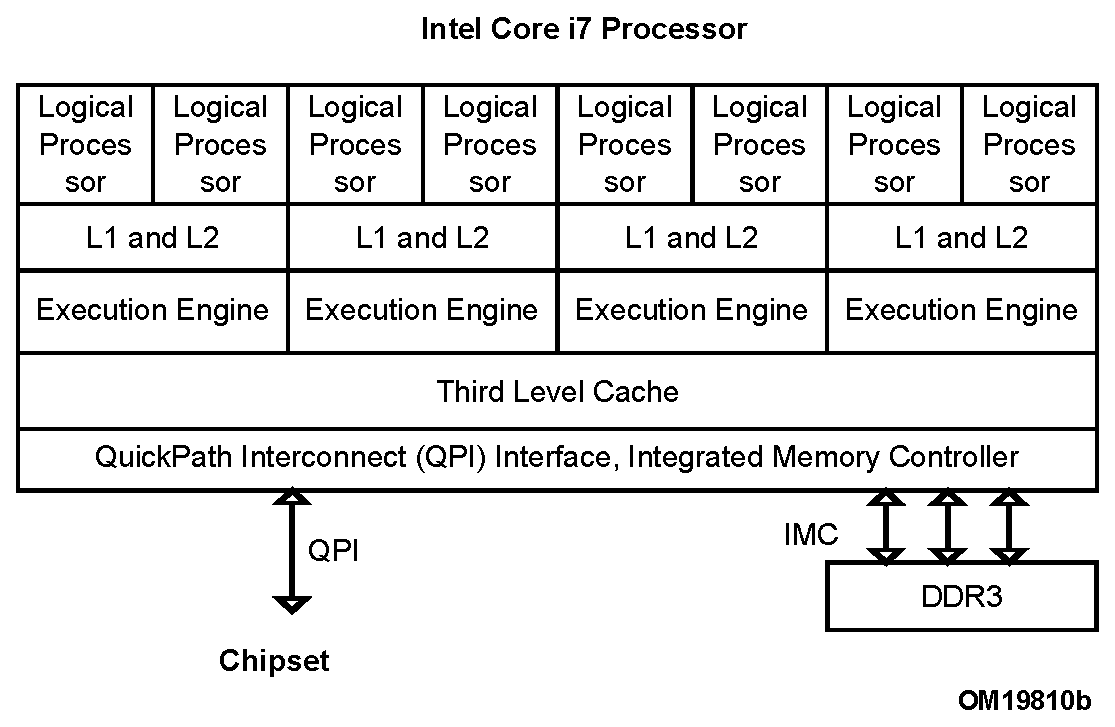
\includegraphics[width=\textwidth]{fig/sandy-bridge-layout.eps}
  \caption{\JWPcpu{} cache organization (taken from \cite{intel2011softdev1})}
  \label{fig:cache-orga}
\end{figure}

The most evident characteristics of the \JWPcpu{} are the four cores (on one
chip) and the uniform distribution of the caches (see figure
\ref{fig:cache-orga}). All caches except for the last--level cache (L3) are
present on each core \cite{fog11}. The CPU's \emph{performance monitoring unit}
(PMU) appears---because of its central importance---in a separate chapter
(\ref{sec:pmu}). A short overview of the key features follows
\cite{intel2011spec}:

\begin{itemize}

\item Number of cores: 4

\item CPU clock speed: \SI{3.4}{\giga\hertz}

\item L1 cache of \SI{64}{\kibi\byte} per core\cite{intel2011softdev1}

\item L2 cache of \SI{256}{\kibi\byte} per core\cite{intel2011softdev1}

\item shared L3 cache of \SI{8}{\mebi\byte}\cite{intel2011softdev1}

\end{itemize}


%-  PMU  -----------------------------------------------------------------------
\JWlthree{Performance Monitoring Unit}
\label{sec:pmu}

The CPU's \emph{Performance Monitoring Unit} (PMU) is present since the
Intel\TReg{} Pentium processor. It is able to monitor several of the
CPU's performance parameters while the system is running. Originally meant for
tuning system and application performance \cite{intel2011softdev3b}, it is
mostly used by compiler developers.

In prior work \cite{bellosa2000benefits,snowdon2010operating,
weissel2002process,kellner03tempcontrol,bertran2010decomposable} some of these
performance events have proved to be somehow related to the power consumption of
the CPU. The selection of the events and the degree of their correlation to
energy highly varies among CPUs, or at least CPU microarchitectures. Therefore,
selection and fitting have been done again for the Intel\TReg{} San\-dy Bridge
microarchitecture and in particular the \JWPcpu{}.

By examining the processor user's manual \cite{intel2011events} approximately
184 events have been found available and usable. Because the CPU is only able to
count eight (four in Hyper--threading \cite{HT} mode) user--programmable
performance events simultaneously \cite{intel2011softdev1} the most useful
events have to be selected. In addition to the eight (four) events, the CPU
provides three counters for fixed events, which will be counted in any case:
\JWctr{CPU\_CLK\_UNHALTED.REF\_TSC}, \JWctr{CPU\_CLK\_UNHALTED.THREAD} and
\JWctr{INST\_RETIRED.ANY}.

The selection, configuration and usage of these performance event counters is
done via special \emph{model specific registers} (MSRs)
\cite{intel2011softdev3b}. In this work a more high--level approach via the
\JWpn{perf\_event}-API (unofficial documentation at
\cite{weaver2011perfevents}) of newer Linux Kernels and \JWTlibpfm{} (see
chapter \ref{sec:standard-software}) has been used.


%-  architectural differences  -------------------------------------------------
\JWlthree{Architectural Differences among San\-dy Bridge and its Predecessors}

The Intel\TReg{} \emph{San\-dy Bridge} microarchitecture is a further
development of the Core and Nehalem architectures \cite{fog11}. Among other
simplifications of the branch prediction unit, the special loop predictor has
been discontinued presumably to reduce the overall pipeline length and to
minimize the misprediction penalties \cite{fog11}. For speed--improvements a
micro--operation ($\mu$op) cache and macro--operation fusion have been
introduced \cite{fog11}.

% vim: set spell spelllang=en_us fileencoding=utf8 : syntax spell toplevel :
